\begin{figure}[ht]
    \centering
    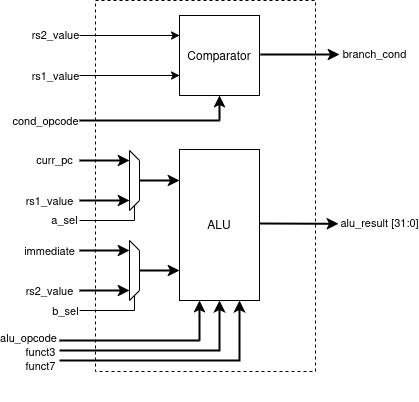
\includegraphics[scale=0.4]{IE_BD.png}
    \caption{A block diagram for the execution stage}
    \label{fig:IE_BD}
\end{figure}

\subsection{Instruction analysis and Execution}
With the previous information extrapolated from the instruction, there is now the need to elaborate the incoming values stored in their relative registers, by performing the needed operation type.
The Instruction Execute stage, implemented in the simplest way possible can be described in VHDL with two main blocks:
\begin{itemize}
\item \textbf{Comparator}: takes two 32-bit inputs and returns a boolean value indicating wether or not the comparison between the two inputs follow a decided criteria. This block is dedicated to the branch-type instructions, that may end in an instruction jump.
\item \textbf{Arithmetic-Logic Unit}: performs all other arithmetic and logic operations, while also handling shifts. When coding this block it has to be taken into account that both signed and unsigned operations have to be performed. For this reason the inputs of each multiplexer will be casted as unsigned at first (to match for the immediate values already being unsigned) and then casted correctly afterwards. 
\end{itemize}
Starting from the ALU, being the most complex of the two, the necessary steps to take before the description is to understand what type of operation has to be done for each core instruction. As said earlier, some of them can be recognized for both the presence of \emph{funct3} (bit 14 to 12) and \emph{funct7}, in case of R-type onstructions, or just \emph{funct3}. As specified in the base RV32I manual, the univocal codes for the basic core instructions are listed in table \ref{table:core_instr}, from which it is easy to notice that the actual purpose of \emph{funct7} is to switch between addition and substraction, since they are encoded as "000", or between logic and arithmetic right shift (in the table SRA and SRL). A simple solution could be editing the behavior of the decoder to have it look at the sixth bit of \emph{funct7} and have all subtractions encoded as "010", as it would happen for SLT, and similarly for SRL and SRA. This solution would remove the necessity for \emph{funct7} and shrink the necessary opcode for the ALU to 3 bits. However, that portion of the instruction, seemingly unnecessary for RV32I, comes useful when implementing floating-point instructions and multiplications, hence the most flexible solution, however complex, is to make the decoder return \emph{funct7} and have the ALU taking it into account when switch between operations.
With this in mind now the decoder can be edited to return \emph{funct7} when treating opcodes mapped as OP, and some instances of OP-IMM when treating shifts.With this being said, it is decided that the ALU can switch operation by taking into account, in order of importance: the instruction class, \emph{funct3} and, to maintain flexibility for future modifications, \emph{funct7}.


If the ALU can be defined as a big case statement as for the decoder, Table \ref{table:core_instr} may help to simplify the code, in fact some observations can be already made fro basic optimizations:
\begin{enumerate}
\item Many instructions expect the ALU to perform an addition, thus if the architecture of the block is written as a case statement, \emph{the addition can be performed if no other case applies}.
\item All load and store operations require \emph{funct3} to be used later during WriteBack stage because they may operate with less than 32 bits, thus it can be useful to \emph{pass it down to the latest stages of the datapath}.
\item Shift operations using immediates are encoded as I-type but they just need five bits indicated as \emph{shamt} (shift amount), for shifting more than 32-bits would not make any sense. While this does not affect SLLI and SRLI, the presence of \emph{funct7} rises a problem with SRAI. \emph{Shifts with immediates need to filter part of the second operand}.
\end{enumerate}
The code for the ALU will thus check the operation class, funct3 and funct7 in the latter sequence. Also, the block will return a new logic vector, named \emph{ls{\_}class} which, in case of L/S operations, will serve the WB stage to identify the length to which the instruction is operating, being it 8, 16 or 32 bits. Notes Code Source \ref{code:IE_ALU} shows a VHDL implementation that follows said constraints.\\
While the code may seem wrong for defining the combinatory logic inside a clock-sensitive process, it is to keep in mind that for now the datapath is not pipelined, and the process defines the behavior of the input of a register. Later, when the inter-stage register of the pipeline will be implemented, the correct way of defining the ALU, and other combinatory blocks that may come, is to define them inside process that are instead input-sensitive.\\
Branches only require a comparison and just need a single signal to indicate wether or not a jump can happen. From the RV32I instruction table, the remaining core instructions  to implement are indicated in Table \ref{table:core_instr} as BRANCH class instrutions. As it has been for the ALU, the table leads us to a case statement, much simpler than before due to just having to look at \emph{funct3}; A much more self-explanatory architecture can be seen in Source Code \ref{code:IE_comparator}.\\
Finally, the IE (Shown as Source Code \ref{code:IE_code}, much easier to visualize in Figure \ref{fig:IE_BD}) can be "assembled" by routing inputs and outputs of each block, and by also coding multiplexers for the operand selection:

\begin{minted}[fontsize=\footnotesize]{vhdl}
alu_mux_a   <= rs1 when a_sel = '1' else curr_pc;
alu_mux_b   <= rs2 when b_sel = '1' else imm_se;
\end{minted}

\subsection{Simulation}
With the current initialization files for the IM, only a small amount of instructions are going to be tested, for this reason the new file should contain each existing tipology, possibly testing the ones that use \emph{funct7} while also implementing jumps and branches, possibly with a loop so that the next stages can be easily tested for inconsistencies or error that may stop the code from running.
The new initialization could become:

\begin{minted}{text}
memory_initialization_radix = 16;
memory_initialization_vector =
000100b7,   --> lui x1, 0x10
00408113,   --> addi x2, x1, 4
002081b3,   --> add x3, x1, x2
0030a223,   --> sw x3, 4(x1)
0040a203,   --> lw x4, 4(x1)
404182b3,   --> sub x5, x3, x4
0000006f,   --> jal x0, 0 
fe108ee3;   --> beq x1, x1, -8
\end{minted}

The tesbench, following the step-by-step assembly of the whole datapath proposed in the ID section, can be built using a copy of the earlier code with the IE as an addition.\\
Now when running a behavioral simulation of the testbench it should be expected that: the first instruction is going to be encoded with \emph{op{\_}class} = "00010", while setting \emph{b{\_}sel} and pulling down \emph{a{\_}sel}, leaving \emph{alu{\_}result}=16; The second one should be acting the same, with the difference being that the output from the ALU will be 4 since x1 can not yet be read; The following load, store and jump instruction should be performing an addition, easy to notice from the ALU's output; The subtraction should instead change \emph{funct7} and the last one should have the comparator set its only output:

\begin{figure}[ht]
    \centering
    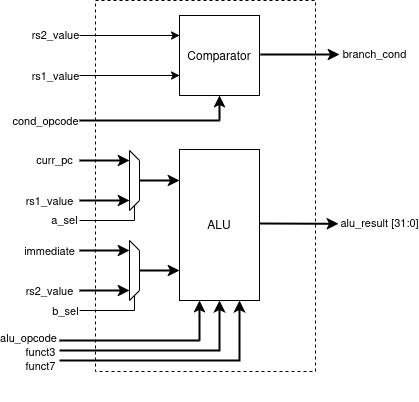
\includegraphics[scale=0.4]{IE_BD.png}
    \caption{A block diagram for the execution stage}
    \label{fig:IE_BD}
\end{figure}
\begin{figure}[ht]
    \centering
    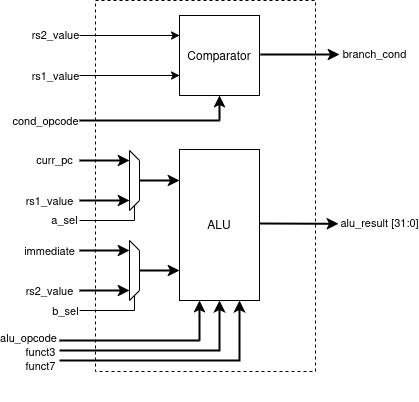
\includegraphics[scale=0.4]{IE_BD.png}
    \caption{A block diagram for the execution stage}
    \label{fig:IE_BD}
\end{figure}
\begin{figure}[ht]
    \centering
    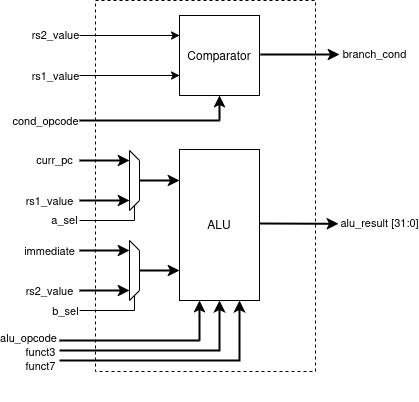
\includegraphics[scale=0.4]{IE_BD.png}
    \caption{A block diagram for the execution stage}
    \label{fig:IE_BD}
\end{figure}

